% !TEX root = ../notes.tex

\section{Introduction to PDEs}
A differential equation that contains, in addition to the dependent variable and independent variables, one or more partial derivatives of the dependent variable is called a partial differential equation.\\

In general it may be written in the form,
\begin{equation}
  f(x, y, \dots, u, u_x, u_y, \dots, u_{xx}, u_{yy}, \dots) = 0
\end{equation}
involving several of the $x, y, u_{x}, u_{xx}$ terms. Note that the notation $u_x = \pd{u}{x}$.\\

When we consider a PDE, we also consider it in a suitable domain. For us, the domain, $D$, will just be some domain of $\R^n$ in the variables $x, y, \dots$. A solution of this equation will be a function $u = u(x, y, \dots)$ which satisfy $(1)$. We call the order of the PDE the highest order partial derivative appearing the equation.
\begin{eg}
  $u_{xxy} + xu_{yy} + 8u = 8y$ is a third order PDE.
\end{eg}

\begin{ndefi}[Linear]
  We call a PDE linear if it is linear in the unknown function and all it's derivatives. For example,
  $$ yu_{xx} + 2xyu_{yy} + u = 1 $$
\end{ndefi}

and we have a further characterisation, called quasi-linear,

\begin{ndefi}[Quasi-Linear]
  A PDE is quasi linear if it linear in the highest-orderderivative of the unknown function,
  $$ u_xu_{xx} + xuu_y = \sin y $$
\end{ndefi}

and furthermore, an equation that isn't linear is non-linear. IN this course we will consider mainly second order linear PDEs. The most general of these can be written as,
$$ \sum_{i, j = 1}^n A_{ij}u_{x_ix_j} + \sum_{i=1}^n B_iu_{x_i} + F_u = G $$
where we assume that $A_{ij} = A_{ji}$, we also assume that $B_i$, $F$ and $G$ are functions of the $n$ independent variables $x_i$. If $G = 0$, then we have a homogenous PDE; otherwise it's non-homogenous.\\

If we consider an $n^{th}$ order ODE, then what we end up with is a solution depending on $n$ arbitrary constants. A similar thing applies to PDEs, but they are $n$ arbitrary functions. To illustate, we solve $u_{xy} = 0$, where first we integrate wrt $y$, and we get $u_x = f(x)$ and then integrate wrt $x$ and we get $u(x, y) = g(x) + h(y)$ where $g$ and $h$ are arbitrary functions.

\subsection{Mathematical Problems}
A mathematical problem is PDE along with some supplimentary conditions on that PDE. the conditions may be intial conditions that are of the form $u(x, 0) = f(x)$ or boundary conditions which depends on the boundary. Let us take the example of the following PDE,
$$ u_t - u_{xx} = 0 $$
Then an initial conditions for this PDE may be $u(x, 0) = \sin x$ and if we consider it on some boundary $0 \le x \le \ell$ some boundary conditions may be $u(0, t) = 0$ and $u(\ell, t) = 0$ for some $t \ge 0$ (This example is the heat equation for a rod of length $\ell$). This problem is known as an initial boundary problem. Sometimes we have more conditions that specify the problem, for example some conditions on the derivative. If we have a boundary that is not bounded, then sometimes we won't have boundary conditions and then we have a initial-value problem or a Cauchy Problem. \\

Finally, we say that a problem is well posed if,
\begin{enumerate}
  \item Existence, there is at least one solution
  \item Uniqueness, there is at most one solution
  \item Continuity, the solutions depends continuously on the data. A small input in the input data must reach a small change in the output data.
\end{enumerate}

\subsection{Linear Operators}
An operator is a mathematical rule which when applied to a function produces another function. For example where,
\begin{align*}
  L[u] &= \pdd u x + \pdd u y\\
  M[u] &= \pdd u x - \pd u x + x\pd u x
\end{align*}
then we say that $L = \pdd {} x + \pd {} y$ and $M = \pdd {} x - \pd {} x + x\pd {} x$ are the differential linear operators. We note a few things before a formal definition, if we have linear operators $L$ and $M$, then $(L + M)[u]$ is a linear operator and $(L + M)[u] = L[u] + M[u]$. Furthermore, we can do something similar with $LM[u] = L(M[u])$. In general, here is the definition,

\begin{nlemma}
  Let $L, M$ and $N$ be linear operators. In general, a linear operator satisfies the following,
  \begin{itemize}
    \item $L + M = M + L$ (commutativity of addition)
    \item $(L + M) + N = L + (M + N)$ (associativity of addition)
    \item $L(MN) = (LM)N$ (associativity of multiplication)
    \item $L(c_1M + c_2N) = c_1LM + c_2LN$ (distributivity)
  \end{itemize}
  and for Linear Differential operators with constant coefficients, we have that $LM = ML$.
\end{nlemma}

Now consider a linear second order PDE,
$$A(x, y)u_{xx} + B(x, y)u_{xy} + C(x, y)u_{yy} + D(x, y)u_x + E(x, y)u_y + F(x, y)u = G(x, y)$$
then if we let,
$$ L = A(x, y)\pdd{}{x} + B(x, y)\pdxy u + C(x, y)\pdd{}{y} + D(x, y)\pd{}{x} + E(x, y)\pd{}{y} + F(x, y) $$
be a linear differential operator, then we can write $Lu = G$ and that is our PDE.\\

Let $v_1, v_2, \dots, v_n$ be $n$ functions satisfying
$$ L[v_j] = G_j $$
 for $j$ running from $1$ to $n$. Let $w_1, w_2, \dots, w_n$ be $n$ functions where $L[w_j] = 0$ for $j$ running from $1$ to $n$. If we let $u_j = v_j + w_j$ then $u=  \sum_{j=1}^n u_j$ this is called the principle of linear superposition.\\

\noindent
If we consider $u_{tt} - c^2u_{xx} = G(x, t)$ if we solve this for $0 < x < L$ where $u(x, 0) = g_1(x)$ and $u_t(x, 0) = g_2(x)$ for $0 \le x \le L$ and $t \ge 0$. We also have boundary conditions $u(0, t) = g_3$ and $u(L, t) = g_4$. We can write this in the form, $l[u] = G$ and $m_1[u] = g_1$ and $M_2[u] = g_2$ and $M_3[u] = g_3$ and finally $M_4[u] = g_4$. We can now decomopse this into four different problems.
\begin{itemize}
  \item $L[u] = G$, $M_1[u] = 0$, $M_2[u_1] = 0$, $M_3[u_1] = 0$ and $M_4[u_1] = 0$
  \item $L[u_2] = 0$, $M_1[u_2] = g_1$, $M_2[u_2] = 0$, $M_3[u_1] = 0$ and $M_4[u_1] = 0$
  \item $L[u_2] = 0$, $M_1[u] = 0$, $M_2[u_1] = g_2$, $M_3[u_1] = 0$ and $M_4[u_1] = 0$
  \item $L[u_3] = 0$, $M_1[u] = 0$, $M_2[u_1] = 0$, $M_3[u_1] = g_3$ and $M_4[u_1] = 0$
  \item $L[u_3] = 0$, $M_1[u] = 0$, $M_2[u_1] = 0$, $M_3[u_1] = 0$ and $M_4[u_1] = g_4$
\end{itemize}
and then solve the above and then add them together via the linear superposition.

\subsection{Boundary Conditions}
Assume we have $u_{xx} + u_{yy} = 0$ with a domain and boundary,
% add boundary diagram

\begin{figure}[!ht]
\centering
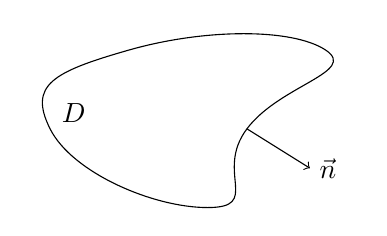
\begin{tikzpicture}
  \draw [black] plot [smooth cycle, tension=1] coordinates {(0,0) (1,1) (3.5,1) (2.5,0) (2,-1)};
  \draw[->] (2.5, 0) -- (3.3, -0.5) node[right] {$\vec n$};
  \node at (0.3, 0.2) {$D$};
\end{tikzpicture}
\end{figure}

where $u(x, y) = f(x, y)$ along the boundary of $D$, then we have a Dirichlet Boundary condition. If $\pd u x = h(x, y) \to \partial D$ is a Neumann boundary condition. We can also have $\pd u {\vec n} = \nab u \cdot \vec n$. If we can split the boundary into two then we can have a mixed type boundary condition; $u(x, y) + \pd u n = h(x, y)$ this is called a Robin Boundary condition.

\begin{exercise}
  Prove that $\R^3$, gradient, curl and divergence are all linear differential operators, ie. prove that,
  \begin{align*}
    L(f + g) &= L(f) + L(g)\\
    L(cf) &= cL(f)
  \end{align*}
  where $c \in R^3$ and $f, g$ are elements.
\end{exercise}
\begin{exercise}
  Solve,
  $$ 5u'' - 4u' + 4u = e^x\cos x $$
  for a solution $u(x) = \frac{1}{6}e^x\sin x + c_1e^{\frac{2}{5}x}\cos \frac{4x}{5} + c_2e^{\frac{2x}{5}}\sin \frac{4x}{5}$
\end{exercise}


We now define classical solutions. Assume we have a PDE,
$$ A\pdd u x + B\pdxy u + C\pdd u y = D $$
with a solution, $u(x, y)$, for a classical solution we need this solution continuously second differentiable.

\begin{ndefi}[Smooth]
  A function is smooth if it can be differentiated sufficiently enough.
\end{ndefi}

If the PDE has order $n$, then a solution has class $\mathcal{C}^n$. If we consider
$$ \pd u t + k\pdd u x = 0 $$
A solution is classical if $u(x, t)$ is differentiable by all th variables $n$ times.

\section{First Order Linear and Nonlinear waves}
We want to solve,
$$ \pd u t = 0 $$
for $u(x, t)$. We can integrate both sides wrt time,
$$ \int_0^t \pd u s \, ds = 0 $$
and so we see $u(x, t) - u(x, 0) = 0$ and so $u(x, t) = f(x)$ where $f(x)$ is defined by the IC. For this to be classical $f(x) \in \mathcal{C}^1$. If $f(x) = x$, then we get $u(x, t) = xt + f(x)$ where $f(x) \in \cc^1$.\\

If we want to solve $u_t = x - t$, then $u(x, t) = xt - \frac{1}{2}t^2 + f(x)$, or $u_x + tu = 0$ then we can use an integrating factor and then get $\pd u t (e^{tx}u) = 0$ and so $u(x, t) = e^{-tx}f(t)$ where $f(t) \in \cc^1$.\\

Next let us add another term,
$$\pd u t + c\pd u x = 0$$
where $c$ is a constant. This is a transport equation, and the solution is a travelling wave. This models a uniform fluid flow with speed $c$ subject to the condition $u(x, t_0) = f(x)$. We aim to reduce this to an ODE. Let us introduce $\xi = x - ct$ (the characteristic variable), then $u(x, t) = v(\xi, t) = v(x - ct, t)$. Let us take partial derivatives,
$$ \pd u t = \pd v t + \pd v \xi \pd xi t = v_t - cv_\xi$$
and
$$ \pd u x = \pd v \xi \pd \xi x = v_\xi $$
and so we get, $v_t - cv_\xi + cv_\xi$ and so $v_t = 0$. Hence, $v = v(\xi) = v(x - ct)$.

Now let us put this more formally,
\begin{nprop}
   If $u(x, t)$ is a solution to the PDE
   $$\pd u t + c\pd u x = 0$$
   defined on all $\R^2$. Then, $u(x, t) = v(x - ct)$ where $v(\xi)$ is a $\cc^1$ function of the characteristic variable $\xi = x - ct$.
\end{nprop}

Now for an example,
\begin{eg}
  Solve,
  $$ \pd u t + 2\pd u x = 0 $$
  subject to $u(x, 0) = \frac{1}{1 + x^2}$. To solve this, consider the characteristic variable, $\xi = x - 2t$, then we can represent the solution in the form $v(x - ct)$. To see this we represent the PDE as,
  $$ \pd u t = -v_\xi + v_t $$
  $$ \pd u x = v_\xi\xi_x = v_\xi $$
  and so we can plug these in and get,
  $$ v_t = 0 $$
  and so $v = v(x - 2t)$. Now we plug in the IC and get that $v(x) = \frac{1}{1 + x^2}$ and so $v = \frac{1}{1 + (x - 2t)^2}$ and hence, $u(x, t) = \frac{1}{1 + (x - 2t)^2}$.
\end{eg}

Let's go one step further with the transport equation with decay.
$$ \pd u t + c \pd u x + au = 0 \qquad a > 0 $$
\begin{eg}
  We want to again use characteritics, so let $\xi = x - ct$ and so $u(x, t) = v(\xi, t) = v(x - ct, t)$. Then we get $u_t = -cv_\xi + v_t$ and $u_x = v_\xi$. Hence again we get that $\pd v t + av = 0$, solve by an integrating factor of $e^{at}$ and conclude that $\pd{}{t}(ve^{at}) = 0$ and so $v = e^{-at}f(\xi)$. We can hence conclude that $v(\xi, t) = e^{-at}f(\xi)$ and $u(x, t) = e^{-at}f(x - ct)$. $f \in \cc^1$.
\end{eg}

\begin{exercise}
  Solve,
  $$ \begin{cases}
    \pd u t - 3\pd u x = 0\\
    u(x, 0) = e^{-x^2}
  \end{cases} $$
  $$ \begin{cases}
    \pd u t + 2\pd u x = 1\\
    u(x, 0) = e^{-x^2}
  \end{cases} $$
\end{exercise}

Now let us adapt this such that $c = f(x)$, a non-uniform transport equation. It is of the form,
$$ \pd u t + c(x)\pd u x = 0 $$
To use the method of characteristics, we would like to know how the solution varies along a curve in the $(x, t)$ plane. We can parametrise any curve and so let us let $h(t) = u(x(t), t)$ and we want to measure the rate of change as the solutions moves along some curve in the plane. Now we take the derivative of $h(x)$ wrt time,
$$ \pd h t = \pd u t (x(t), t) + \pd u x(x(t), t)\di x t $$
Now we assume that $\di x t = c(x)$, then we can conclude that, $$\pd u t = \pd u t (x(t), t) + c(x) \pd u x(x(t), t)$$
and since we are assuming that the curve is a solution, then this is just our PDE. Hence, $\pd u t = 0$. The solution is constant along the characteristic.

\begin{ndefi}[Characteristic Curve]
  The graph of a solution $x(t)$ to the autonomous ODE $\di x t = c(x)$ is called the characteristic curve. For the transport equation with wave speed $c(x)$.
\end{ndefi}

\begin{nprop}
   Solutions to the linear transport equation $u_t + c(x) u_x = 0$ are constant along characteristic curves.
\end{nprop}

Hence, from $\di x t = c(x)$, we can find a characteristic curve for the PDE; if we integrate it then we can say that $\b(x) = \int \frac{dx}{c(x)}$, then we can achieve that $\b(x) = t + c$ and so we say that $\xi = \b(x) - t$.

\begin{eg}
  Solve
  $$ \pd u t + \frac{1}{1 + x^2}\pd u x = 0 $$
  using the method of characteristics.
\end{eg}

\subsection{Quasi-Linear equations and methods of MoC}
We can write
$$ F(x, y , u, u_x, u_y) = 0 \qquad (x, y) \in D \subset \R$$
Then if we write $u_x = p$ and $q = u_y$. Then this solution is quasi-linear if,
$$ F(x, y, u, p, q) = 0 $$
is quasi-linear if the PDE is linear in first partial derivatives of the unknown function $u(x, y)$. We can write the most general form as,
$$ a(x, y, u)\pd u x + b(x, y, u)\pd u y = c(x, y, u) $$
Some examples are,
$$ x(y^2 + u)u_x - y(x^2 + u)u_y = (x^2 - y^2)u $$
We call a PDE semi-linear if it further satisfies $a$ and $b$ being independent of $u$,
$$ a(x, y)u_x + b(x, y)u_y = c(x, y, u) $$
For example,
$$ xu_x + yu_y = u^2 + x^2 $$
We call a PDE linear if it is linear in each of the variable,
$$ a(x, y)u_x + b(x, y)u_y + c(x, y)u = d(x, y) $$
If $d(x, y) = 0$ we get a homogenous first order PDE and if $d(x, y) \ne 0$ then we have a non-homogenous first order PDE. For example, a homogenous PDE,
$$ xu_x + yu_y - nu = 0 $$
and a non-homogenous PDE,
$$ nu_x + (x + y)u_y - u = e^x $$
More generally, these are geometric surfaces described by $f(x, y, z, a, b) = 0$ and if this exists, then the solution is complete. We can also reduce $a$ and $b$ out. A solution can be written as $f(\phi, \psi) = 0$ where $\phi, \psi \in \R^3 \to \R^3$.

\begin{eg}
  Show that a family of spheres $x^2 + y^2 (z - c)^2 = r^2$ satisfies the first order linear PDE $yp - xq = 0$ where $p = z_x$ and $q = z_y$.
\end{eg}

\begin{exercise}
  Show that the family of spheres $(x - a)^2 + (y - b)^2 + z^2 = r^2$ satisfy $z^2(p^2 + q^2 + 1) = r^2$ where $p = z_x$ and $q = z_y$.
\end{exercise}

\begin{nthm}[]
  If $\phi = \phi(x, y, z)$ and $\psi = \psi(x, y, z)$ are two given functions of $x$, $y$ and $z$ and if $f(\phi, \psi) = 0$ where $f$ is an arbitrary function of $\phi$ and $\psi$. Then $z = z(x, y)$ satisfies a first order PDE,
  $$ p\pd{(\phi, \psi)}{(y, z)} + q\pd{(\phi, \psi)}{(z, x)} = \pd{(\phi, \psi)}{(x, y)} $$
  where
  $$ \pd{(\phi, \psi)}{(x, y)} = \left| \begin{matrix}
    \phi_x & \phi_y \\ \psi_x & \psi_y
  \end{matrix} \right| $$
\end{nthm}
\begin{proof}
  Let $f(\phi, \psi) = 0$ and now let us differentiate by $x$ and $y$, then,
  $$ \pd f \phi \pd \phi x + \pd f \phi\pd \phi z \pd z x + \pd f \psi \pd \psi x + \pd f \psi \pd \psi z \pd z x = 0 $$
  and simplify,
  $$ \pd f \phi \left( \pd \phi x + p\pd \phi z \right) + \pd f \psi \left(\pd \psi x + p\pd \psi z\right) = 0 $$
  and now we do the same thing for $y$,
  $$ \pd f \phi \left( \pd \phi y + q\pd \phi z \right) + \pd f \psi \left( \pd \psi y + q\pd \psi z\right) $$
  and now let us write these in matrix form,
  % matrices
  There is a non-trivial solution is and only if the  determinant matrix is zero. If we calculate this determinant we get the solution of the PDE.
\end{proof}

If we consider a PDE of the form,
$$ a(x, y, u)u_x + b(x, y, u)u_y - c(x, y, u) = 0 $$
If we assume that $z = u$ is a solution surface, then we can define $f(x, y, u) = u(x, y) - u = 0$
% surfaces
Then we can write it as the following,
$$ au_x + bu_y - c = (a, b, c) \cdot (u_x, u_y, -1) = 0 $$
and so we can write it as $\nab u \cdot (a, b, c)$ and so we know that $\nab u$ is normal to the surface and so $(a, b, c)$ must be tangent to the surface and we call the direction of the vector the characteristic direction. Now we seek to parametrise a curve such that $(a, b, c)$ is tangent to the curve. If we paramerise the curve by $(x(t), y(t), u(t))$, then the tangent to the curve will be $(\di x t, \di y t, \di u t) = (a, b, c)$. Now we can find the chateristic curve as we see that
$$ \begin{cases}
  \di x t = a(x, y, u)\\
  \di y t = b(x, y, u)\\
  \di u t = b(x, y, u)
\end{cases} $$
and we can write them as, $\frac{dx}{a(x, y, u)} = \frac{dy}{b(x, y, u)} = \frac{du}{c(x, y, u)} = dt$. Now we move to another theorem,

\begin{nthm}
  The general solution of a first order quasi-linear PDE
  $$ a(x, y, u)\pd u x + b(x, y, u)\pd u y = c(x, y, u) $$
  is $f(\phi, \psi) = 0$ where $f$ is an arbitrary function of $\psi, \phi : \R^3 \to \R^3$, $\phi = c_1$ and $\psi = c_2$ are solution curves of the characteristic equations,
  $$ \frac{dx}{a} = \frac{dy}{b} = \frac{du}{c} $$
  and $\phi(x, y, u) = c_1$ and $\psi(x, y, u) = c_2$ are the family of characteristic curves.
\end{nthm}
\begin{proof}
  Let $\phi(x, y, u) = c_1$ and $\psi(x, y, u) = c_2$. From the first, we can say that,
  $$ d\phi = \phi_x dx + \phi_ydy + \phi_udu = 0 $$
  and so,
  $$ \di \phi t = \phi_x \di x t + \phi_y \di y t + \phi_u\di u t = 0 $$
  and so we get $a\phi_x + b\phi_y + c\phi_u = 0$ and similarly we can get $a\psi_x + b\psi_y + c\psi_u = 0$. ({\color{red} Exercise}). We can now take each of the terms to the right hand side in term and then show that,
  \begin{equation}
    \frac{a}{\pd{(\phi, \psi)}{(y, u)}} = \frac{b}{\pd{(\phi, \psi)}{(u, x)}} = \frac{c}{\pd{(\phi, \psi)}{(x, y)}} \tag{$*$}
  \end{equation}
  and so now from Theorem 2.4, and using the above result $(*)$ we get an expression of the form,
  $$ ap + bq = c $$
\end{proof}